%!TEX program = xelatex

\documentclass[compress]{beamer}
%--------------------------------------------------------------------------
% Common packages
%--------------------------------------------------------------------------
\usepackage[english]{babel}
\usepackage{pgfpages} % required for notes on second screen
\usepackage{graphicx}

\usepackage{multicol}

\usepackage{tabularx,ragged2e}
\usepackage{booktabs}


\usetheme{hri}

\usepackage{tikz}
\usetikzlibrary{mindmap,backgrounds,positioning}

\graphicspath{{figs/}}

%--------------------------------------------------------------------------
% General presentation settings
%--------------------------------------------------------------------------
\title{RGB-D Cameras for Human-Robot Interaction}
\subtitle{~}
\date{\today}
\author{Séverin Lemaignan}
\institute{Centre for Neural Systems and Robotics\\{\Medium Plymouth University}}

%--------------------------------------------------------------------------
% Notes settings
%--------------------------------------------------------------------------
%\setbeameroption{show notes on second screen}

\begin{document}
%--------------------------------------------------------------------------
% Titlepage
%--------------------------------------------------------------------------

\licenseframe{github.com/severin-lemaignan/lecture-rgbd-cameras-hri}

\maketitle

\section*{Overview}
\begin{frame}{Overview}
    \tableofcontents[hideallsubsections]
\end{frame}


%%%%%%%%%%%%%%%%%%%%%%%%%%%%%%%%%%%%%%%%%%%%%%%%%%%%%%%%%%%%%%%%%%%%%%%
%%%%%%%%%%%%%%%%%%%%%%%%%%%%%%%%%%%%%%%%%%%%%%%%%%%%%%%%%%%%%%%%%%%%%%%
%%%%%%%%%%%%%%%%%%%%%%%%%%%%%%%%%%%%%%%%%%%%%%%%%%%%%%%%%%%%%%%%%%%%%%%

\section{3D Perception for HRI}

\imageframe{pr2-baby-3}

\begin{frame}{Situation Assessment}

    \centering
    \includegraphics[width=\textwidth]{spark.pdf}
\end{frame}

\begin{frame}{Why not 2D?}
    3D interpretation of a 2D scene is hard!

    Resorts to fiducial markers

        \centering
        \video{\textwidth}{videos/model3d.webm?autostart&start=22}\\
\end{frame}

\begin{frame}{Perceiving the humans}

Previously,...

\begin{itemize}
    \item face detection
    \item blob detection
    \item motion capture (£10K+)
\end{itemize}

And then, one morning... the Kinect! (\approx£120 pounds)

\end{frame}


%%%%%%%%%%%%%%%%%%%%%%%%%%%%%%%%%%%%%%%%%%%%%%%%%%%%%%%%%%%%%%%%%%%%%%%
%%%%%%%%%%%%%%%%%%%%%%%%%%%%%%%%%%%%%%%%%%%%%%%%%%%%%%%%%%%%%%%%%%%%%%%
%%%%%%%%%%%%%%%%%%%%%%%%%%%%%%%%%%%%%%%%%%%%%%%%%%%%%%%%%%%%%%%%%%%%%%%
\section{RGB-D cameras}

\begin{frame}{RGB-D cameras: many technologies}
    \begin{itemize}
        \item Stereo-vision
        \item Structured light
        \item Speckle decorrelation
        \item Time-of-Flight
        \item (...several other like coded-aperture)
    \end{itemize}
\end{frame}

\imageframe{depthmap}

\imageframe{stereo_head}

\begin{frame}{Stereo-vision: principle}
    \begin{multicols}{2}

    \begin{center}
        \includegraphics[height=0.8\paperheight]{stereo}
    \end{center}

    \begin{align} 
d &= EF + GH \\ 
    &= BF (\frac{EF}{BF} + \frac{GH}{BF})\\ 
    &= BF (\frac{EF}{BF} + \frac{GH}{DG})  \\ 
    &= BF (\frac{BC + CD}{AC})  \\ 
    &= BF \frac{BD}{AC}  \\ 
    &= \frac{k}{z}  \text{, where} \end{align}
        $k = BD \times BF$\\
        $z = AC$
\end{multicols}
\end{frame}

\begin{frame}{Disparity map}

    \only<1>{
    The disparity map is built by:
    \begin{enumerate}
        \item properly aligning the images ({\Medium
    image rectification}), 
        \item looking for the {\Medium disparity} of each pixel between
    the left and right images.
    \end{enumerate}
    }

    \only<2>{
        Pixel disparity: for each {\Medium pixel patch} on the left, by how many pixel the
        same patch is {\Medium shifted} on the right?

        \begin{center}
            \includegraphics[width=0.45\linewidth]{scene_left}
            \includegraphics[width=0.45\linewidth]{scene_right}

            \includegraphics[width=0.45\linewidth]{disparity}
        \end{center}
    }


\end{frame}
\begin{frame}{Issues with stereovision}
    \begin{itemize}
    \item Requires texture $\Rightarrow$ active stereovision
    \item Computation intensive (less of an issue since computations are
        performed on-board)
    \end{itemize}
\end{frame}


\begin{frame}{Active stereo-vision}
    \begin{center}
        \includegraphics[width=0.8\linewidth]{r200}

        \includegraphics[width=0.8\linewidth]{r200_inside}
    \end{center}
\end{frame}

{
    \paper{Source:
    http://www.hackengineer.com/structured-light-vs-microsoft-kinect/}
    \begin{frame}{Structured light}
        \centering
        \only<1>{
            \begin{multicols}{2}
                \includegraphics[height=0.75\paperheight]{structured_light}



                \includegraphics[width=0.8\columnwidth]{structured_light_gray_code}

                Gray code
                \vspace{1cm}

                \includegraphics[width=\linewidth]{f200_module_simple}
\end{multicols}
}
        \only<2>{

            \video{0.8\linewidth}{videos/structured_light.mp4}
        }
        \only<3>{


            \includegraphics[width=0.8\linewidth]{structured_light_schema}
        }
        \only<4>{

            \video{0.8\linewidth}{videos/structured_light.mp4}

            \begin{table}[htpb]
                \centering
                \begin{tabular}{ccc}
                    & {\Medium Yellow} & {\Medium Red} \\
                    Gray code & 110100111 & 010000111 \\
                    Projector col. & 314 & 250 \\
                    Camera col. & 335 & 392 \\
                    {\Medium Disparity} & 335-314=21 & 392-250=142 \\

                \end{tabular}
            \end{table}
        }

    \end{frame}
}

\begin{frame}{Structured light cameras}
    \begin{center}
        \includegraphics[width=0.4\linewidth]{f200}
        \includegraphics[width=0.6\linewidth]{f200_module}
    \end{center}
\end{frame}


{\fullbackground{kinect360}
\begin{frame}{Speckle decorrelation}


\end{frame}
}

\imageframe[color=black]{kinect_pattern}
\imageframe[color=black]{kinect_pattern2}

\begin{frame}{Multiscale pattern}
    \begin{center}
        \includegraphics[width=0.8\linewidth]{multiscale_kinect_pattern}\\
        \includegraphics[width=0.5\linewidth]{kinect_pattern2}

    \end{center}
\end{frame}

{
\paper{Image source: Wikipedia}
\begin{frame}{Time-of-Flight cameras}
    \begin{center}
        \includegraphics<1>[width=0.8\linewidth]{kinect_xbox_one}

        \includegraphics<2>[width=0.7\linewidth]{tof2}

        \includegraphics<2->[width=0.7\linewidth]{tof1.pdf}

        \only<3->{
            $t_D = 2 \cdot \frac{D}{c} = 2 \cdot \frac{2.5m}{300000000\frac{m}{s}} = 0.00000001666s = 16.66ns$
        }
        \only<4>{
            $D = \frac{1}{2} \cdot c \cdot t_0 \cdot \frac {S2} {S1 + S2}$
        }
    \end{center}
\end{frame}
}

\begin{frame}{Comparison of cameras}
    \begin{table}[]
        \centering
        \scriptsize
        \begin{tabular}{@{}lllll@{}}
            \toprule
                             & Kinect 360 (v1)        & Kinect One (v2)   \\ \midrule
            {\Medium Range}            & 0.6m -- \textgreater5m & 1.37m -- 8m?      \\
            {\Medium Price (new)}      & £230                   & £118               \\
            {\Medium Depth resolution} & 640x480px, 11bits      & 512x424px, 13bits  \\
            {\Medium Libraries}        & libfreenect/OpenNI1    & libfreenect2       \\
            {\Medium horizontal FoV}   & 57                     & 70                 \\
            {\Medium vertical FoV}     & 43                     & 60                 \\
            {\Medium Microphones?}     & 4                      & 4                 \\ \bottomrule
        \end{tabular}
        \begin{tabular}{@{}lllll@{}}
            \toprule
                             & Intel RealSense SR300 & Intel RealSense R200        \\ \midrule
            {\Medium Range}            & 0.2m – 1.6m           & 0.6m -- 3.5m (10m outdoors) \\
            {\Medium Price (new)}      & £66 & £66                         \\
            {\Medium Depth resolution} & 640x480               & 640x480                     \\
            {\Medium Libraries}        & librealsense   & librealsense         \\
            {\Medium horizontal FoV}   & 77 & 77                          \\
            {\Medium vertical FoV}     & 43 & 47                          \\
            {\Medium Microphones?}     & 2 & 0                           \\ \bottomrule
        \end{tabular}
    \end{table}
\end{frame}

%%%%%%%%%%%%%%%%%%%%%%%%%%%%%%%%%%%%%%%%%%%%%%%%%%%%%%%%%%%%%%%%%%%%%%%
%%%%%%%%%%%%%%%%%%%%%%%%%%%%%%%%%%%%%%%%%%%%%%%%%%%%%%%%%%%%%%%%%%%%%%%
%%%%%%%%%%%%%%%%%%%%%%%%%%%%%%%%%%%%%%%%%%%%%%%%%%%%%%%%%%%%%%%%%%%%%%%


\begin{frame}{Point clouds}
    The (2D) depth image is usually converted to a (3D) point cloud:

    $Z = depthmap(x,y)$

    $X = \frac{x-c_x}{Z-f_x}$

    $Y = \frac{x-c_y}{Z-f_y}$

    with $c_x, c_y$ the optical center of the depth camera and $f_x, f_y$ the focal lenght of the depth camera ({\Medium intrisic parameters} of the camera).
\end{frame}

\imageframe[color=black]{pointcloud}

\begin{frame}{RGB-D registration}
    \begin{center}
        \includegraphics<1>[width=0.45\linewidth]{registration-rgb}
        \includegraphics<1>[width=0.45\linewidth]{registration-depth}

        \includegraphics<2>[height=0.8\paperheight]{stereo}

        \includegraphics<3>[width=0.8\linewidth]{registration-registered}
    \end{center}
\end{frame}

%%%%%%%%%%%%%%%%%%%%%%%%%%%%%%%%%%%%%%%%%%%%%%%%%%%%%%%%%%%%%%%%%%%%%%%
%%%%%%%%%%%%%%%%%%%%%%%%%%%%%%%%%%%%%%%%%%%%%%%%%%%%%%%%%%%%%%%%%%%%%%%
%%%%%%%%%%%%%%%%%%%%%%%%%%%%%%%%%%%%%%%%%%%%%%%%%%%%%%%%%%%%%%%%%%%%%%%

\section{Algorithms for point clouds}

\begin{frame}{Two fundamental algorithms}
\centering
{\Medium ICP}: Iterative Closest Point, \\
{\Medium RANSAC}: RANdom SAmple Consensus 
\end{frame}


\begin{frame}{Iterative Closest Point (ICP)}

    Purpose: align to sets of points -- more precisely: {\Medium iteratively}
    estimate the {\Medium rigid transformation} between two point clouds.

    \only<1>{
    \begin{center}
        \includegraphics[width=\linewidth]{icp}
    \end{center}
    }
    \only<2>{
    \begin{enumerate}
        \item for each point in the source cloud, find the closest point in the target cloud
        \item estimate the transformation, trying to minimize the error
        \item transform the source cloud
        \item iterate
    \end{enumerate}
    }
\end{frame}

{
\paper{Source: PCL documentation}
\begin{frame}{RANdom SAmple Consensus (RANSAC)}
    
    Iterative algorithm that tries
    to {\Medium fit a parametric model} of a point distribution to
    observations. The result is an {\Medium estimation of the model's free
    parameters}.

    \begin{multicols}{2}
    
    \footnotesize
    \begin{enumerate}
        \item take a random subset of the data; assume they are {\Medium inliers}; fit the model;
        \item test the other observations against the fitted model;
        \item if enough points are classified as inliers, return the model; otherwise go to 1.
    \end{enumerate}

    \begin{center}
        \includegraphics[width=0.8\linewidth]{ransac_outliers_plane}
    \end{center}
    \end{multicols}

    \uncover<2>{
        Robust to {\Medium outliers}, but no guarantee of optimality
    }

\end{frame}
}

{
\paper{Source: PCL documentation}
\begin{frame}{Point clouds registration}
    \begin{center}
        \includegraphics<1>[width=\linewidth]{scans}
        \includegraphics<2>[width=0.8\linewidth]{registered}
    \end{center}

    \only<3>{
        Registration $\equiv$ estimating the rigid transformation of the imaging
        sensor between scans.
    }
\end{frame}
}

{
\paper{Source: PCL documentation}
\begin{frame}{Registration algorithm}

        \begin{center}
            \includegraphics[height=0.8\paperheight]{registration_process}
        \end{center}

        \note{
        Iterative technique.

The computational steps for two datasets are straighforward:

\begin{itemize}
    \item from a set of points, identify **interest points** (i.e., **keypoints**)
        that best represent the scene in both datasets;

    \item at each keypoint, compute a **feature descriptor**;

    \item from the set of **feature descriptors** together with their XYZ
        positions in the two datasets, estimate a set of **correspondences**,
        based on the similarities between features and positions;

    \item  given that the data is assumed to be noisy, not all correspondences
        are valid, so reject those bad correspondences that contribute
        negatively to the registration process;

    \item from the remaining set of good correspondences, estimate a motion
        transformation.

\end{itemize}
    }
\end{frame}
}

{
\paper{Source: PCL documentation}
\begin{frame}{Features?}
    \begin{center}
        \includegraphics[width=\linewidth]{good_features}
    \end{center}

    \uncover<2>{
    Good features should be:

    \begin{itemize}
        \item invariant over transformations,
        \item invariant over sampling densing,
        \item robust to noise
    \end{itemize}
}
\end{frame}
}

\begin{frame}{SLAM: Simultaneous Localization And Mapping}

    \begin{center}
        \includegraphics[width=\linewidth]{slam1}
    \end{center}
\end{frame}

\imageframe[color=black]{slam2}
\imageframe[color=black]{slam3}

\begin{frame}{Plane segmentation}
    \centering
    \video{\linewidth}{videos/planar_segmentation.mp4}
\end{frame}

%%%%%%%%%%%%%%%%%%%%%%%%%%%%%%%%%%%%%%%%%%%%%%%%%%%%%%%%%%%%%%%%%%%%%%%
%%%%%%%%%%%%%%%%%%%%%%%%%%%%%%%%%%%%%%%%%%%%%%%%%%%%%%%%%%%%%%%%%%%%%%%
%%%%%%%%%%%%%%%%%%%%%%%%%%%%%%%%%%%%%%%%%%%%%%%%%%%%%%%%%%%%%%%%%%%%%%%

\section{Skeleton Tracking}

\imageframe[color=black]{skeleton/skel1}

{
    \paper{Source: John MacCormick, Shotton et al., CVPR 2011}
    \begin{frame}{Skeleton Tracking}

        \begin{center}
            \includegraphics[width=0.3\linewidth]{skeleton/skel3}
            \includegraphics[width=0.3\linewidth]{skeleton/skel2}
            \includegraphics<2>[width=0.3\linewidth]{skeleton/skel1}
        \end{center}
\end{frame}
}

{
    \paper{Source: John MacCormick, Shotton et al., CVPR 2011}

\begin{frame}{Skeleton estimation}
    \begin{enumerate}
        \item Estimate body parts using a randomized decision forest
        \item Estimate the skeleton
    \end{enumerate}
    \begin{center}
        \includegraphics[width=0.8\linewidth]{skeleton/skeleton_estimation}
    \end{center}
\end{frame}
}

{
    \paper{Source: John MacCormick, Shotton et al., CVPR 2011}

\begin{frame}{Body parts}

    {\Medium Train a decision tree} from \approx 1M samples, computer-generated from
    \approx 100K acquired pairs (depth image, motion capture). This allow
    {\Medium tagging} of body parts in the depth image.

    \begin{center}
        \includegraphics[width=0.8\linewidth]{skeleton/training}
    \end{center}
\end{frame}
}

\begin{frame}{Skeleton}
    \begin{center}
        \includegraphics[width=0.8\linewidth]{skeleton/skel4}\\
        \includegraphics[width=0.8\linewidth]{skeleton/skel5}
    \end{center}
\end{frame}

\begin{frame}{}
    \centering
    What to do with a skeleton?
\end{frame}

\begin{frame}{Cartesian space, joint space}
    \begin{center}
        \includegraphics[width=0.45\linewidth]{skeleton/skeleton}
        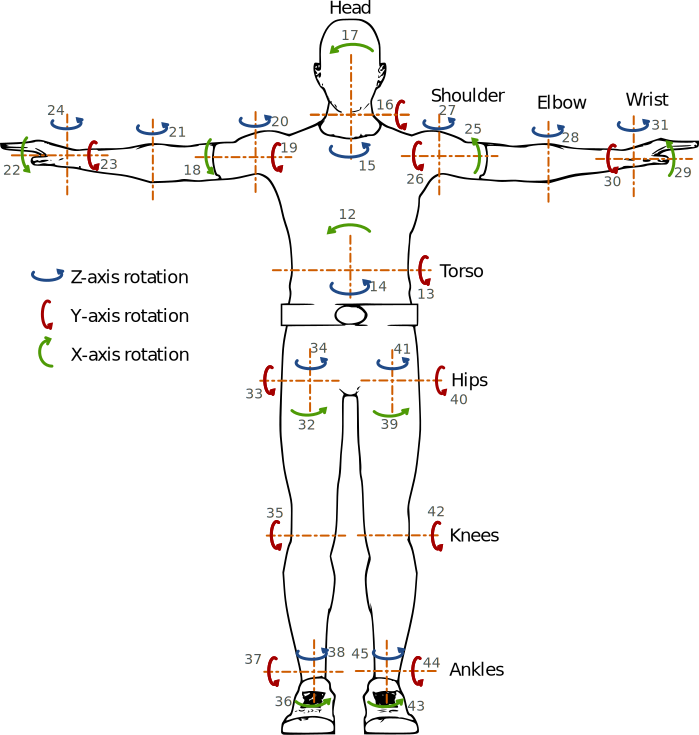
\includegraphics[width=0.45\linewidth]{human_joints}

        Joints values to cartesian positions: {\Medium forward kinematics}
        Cartesian positions to joints: {\Medium inverse kinematics}
    \end{center}
\end{frame}


\begin{frame}{Recognizing postures}
    \centering
    {\Medium Support Vector Machine} (SVM) in joint space
    $\Rightarrow$ supervised training

    \begin{center}
        \includegraphics[width=0.8\linewidth]{svm}
    \end{center}
\end{frame}


{\paper{Images source: http://www.creativedistraction.com}
\begin{frame}{Gestures}
    \begin{center}
        \includegraphics[width=0.5\linewidth]{gesture-ideal}
        \includegraphics<2>[width=0.5\linewidth]{gesture-real}
    \end{center}
\end{frame}
}


{
\paper{Image source: Tdunning, CC-BY 3.0}
\begin{frame}{Hidden Markov Models}
    \begin{center}
        \includegraphics[width=0.5\linewidth]{hmm}
    \end{center}
    \only<1>{
    States: $s_1, s_2,...s_n$ {\scriptsize (eg, step of the gesture)}\\
    Observations: $o_1, o_2,...o_m$ {\scriptsize (eg, hand position)}\\
    State transition probabilities: $a_{ij}$\\
    Output probabilities: $b_{ij}$
}
\only<2>{
    Probabilities are learnt from examples: {\Medium supervised training}

    Very common for {\Medium temporal pattern recognition} (speech, handwriting,
    gestures...)
}

\end{frame}
}

\begin{frame}{Hidden Markov Models}
    We'll leave it here, but for the curious:\\
    \url{http://www.creativedistraction.com/demos/gesture-recognition-kinect-with-hidden-markov-models-hmms/}
\end{frame}

\begin{frame}{Attention}
    \begin{center}
        \includegraphics[width=0.9\linewidth]{field_of_attention}
    \end{center}
\end{frame}


\begin{frame}{}
    \begin{center}
        \Large
        That's all, folk!\\[2em]
        \normalsize
        Questions:\\
        Portland Square A216 or \url{severin.lemaignan@plymouth.ac.uk} \\[1em]

        Slides:\\ \url{github.com/severin-lemaignan/lecture-rgbd-cameras-hri}
    \end{center}
\end{frame}

\end{document}






